\documentclass[11pt]{article}

\usepackage[T1]{fontenc}
\usepackage{amsmath,amssymb,amsthm}
\usepackage{mathptmx}
\usepackage[margin=1in]{geometry}
\usepackage[authoryear,round]{natbib}
\usepackage{booktabs}
\usepackage{tikz}
\usetikzlibrary{arrows.meta,positioning,fit,calc,decorations.pathreplacing}
\usepackage{pgfplots}
\pgfplotsset{compat=1.18}
\usepgfplotslibrary{groupplots}
\usepackage{caption}
\usepackage[hidelinks]{hyperref}
\hypersetup{pdftitle={One Hop or Many: What Solvent Intermediaries Cost a Credit Network}, pdfauthor={Claude Code}}

\theoremstyle{plain}
\newtheorem{proposition}{Proposition}
\theoremstyle{definition}
\newtheorem{definition}{Definition}

\makeatletter
\newcommand{\inputrows}[1]{\@@input #1 }
\makeatother

\title{One Hop or Many: What Solvent Intermediaries Cost a Credit Network}
\author{Claude Code\thanks{Claude Code is an AI agent made by Anthropic, working with the
Microcredit Protocol Project; the research was directed by the project's human operator. See the
disclosure at the end of the paper. Sources, data and code:
\url{https://github.com/scottonchain/microcredit-theory}.}}
\date{Working paper, 5 October 2026}

\begin{document}
\maketitle

\begin{abstract}
\noindent In a credit network, an agent without credit of its own can borrow along chains of trust,
and its borrowing capacity is a maximum flow. A lending protocol on a public blockchain instead lets
an account borrow only from accounts that back it directly, one hop away, so that every default is
charged to an account that chose the borrower. We measure what that restriction costs on synthetic
social graphs (small-world, preferential-attachment and block-model networks of 1,000 accounts), for
a single borrower and in the steady state of repeated loans, against two-hop, three-hop and unbounded
routing and a centralised lender. When credit is spread across the graph, one hop serves 28 to 43\% of
borrowers without credit in the steady state where multi-hop routing serves 83 to 100\%, two hops
close 71 to 86\% of the gap, and one hop needs about twice the issued credit to match two hops. We then show where the gain
comes from. If every intermediary must be able to pay, from its own credit, for what it passes on,
the maximum flow equals the one-hop value exactly. The multi-hop gain therefore comes entirely from
letting accounts relay credit they could not pay for: 40 to 62\% of two-hop volume enters the
borrower through an account without credit, and the default falls on holders who never chose the
borrower. Against Sybil attacks every regime is bounded by its cut and independent of the number of
fake accounts, but the same attack edges extract 3.3 to 7 times as much under multi-hop routing.
\end{abstract}

\medskip
\noindent\textbf{Keywords:} credit networks, maximum flow, length-bounded flow, social collateral,
Sybil attacks, decentralized lending.

% ---------------------------------------------------------------------------------------------
\section{Introduction}

A credit network represents trust as credit lines between pairs of agents. An agent can pay or
borrow from another along any path of lines, and the capacity between two agents is a maximum flow
\citep{defigueiredo2005trustdavis,ghosh2007trust}. \citet{karlan2009trust} show how such networks
let social relationships serve as collateral: an intermediary who vouches for a borrower risks its
relationship with the lender, and a default is paid along the path. \citet{dandekar2011liquidity}
show that on well-connected graphs the network sustains liquidity close to that of a central
currency, and \citet{ramseyer2020liquidity} study agents with aggregate limits.

This paper asks what is lost when the network is restricted to paths of length one. The question
comes from a lending protocol on a public blockchain in which accounts can back borrowers with credit
they hold, and backing received cannot be passed on \citep{conservedcredit2026}. The restriction
keeps every default charged to an account that chose the borrower and can pay for that choice. A
contract over pseudonymous accounts cannot seize social collateral, so an intermediary's promise is
worth only the credit or stake it holds.

We make three contributions.
\begin{itemize}
\item \emph{Measurement.} On small-world, preferential-attachment and stochastic block-model graphs,
  we compare one-hop backing with two-hop, three-hop and unbounded routing and a centralised lender,
  for one borrower on a fresh network and in the steady state of repeated loans. One hop roughly
  halves the liquidity available to borrowers without credit, and two hops recover most of it when
  credit is spread across the graph.
\item \emph{An equivalence} (Proposition~\ref{prop:pathliable}). If every account must be able to
  pay, from its own credit, for all it passes on, the maximum flow into a borrower equals the one-hop
  value. All of the multi-hop gain comes from relaying credit the relay could not pay for, so it
  moves liability to accounts that did not choose the borrower. We measure how much.
\item \emph{Sybil cuts} (Proposition~\ref{prop:sybil}). In every regime, what a set of fabricated
  accounts can extract equals the regime's cut, whatever their number; but the cut is larger under
  multi-hop routing, because an attack edge from an account without credit carries the credit of
  accounts behind it.
\end{itemize}

Section~\ref{sec:model} defines the network and the regimes, Section~\ref{sec:props} proves the two
propositions, Section~\ref{sec:design} describes the experiments, Section~\ref{sec:results} reports
them and Section~\ref{sec:discussion} discusses design choices and limits.

% ---------------------------------------------------------------------------------------------
\section{Model}\label{sec:model}

\paragraph{Accounts and credit.} There are $n$ accounts on an undirected social graph $G=(V,E)$. A
share $q$ of accounts, the \emph{holders}, hold an issued line $L$; the others hold none. A holder's
\emph{free credit} $\varphi(u)$ is its line less what it has already committed. Holders do not borrow.

\paragraph{Trust.} Every edge carries a trust line of $c$ in each direction: a holder will back each
neighbour up to $c$, and the total it backs never exceeds its free credit. In the multi-hop regimes
any account will relay up to $c$ along each of its edges. Lines commit nothing until a loan draws on
them.

\paragraph{Regimes.} A borrower $b$ without credit can draw the following maximum.

\begin{definition}[Regimes]\label{def:regimes}
\begin{itemize}
\item \emph{One-hop:} $\sum_{u\in N(b)}\min\{c,\varphi(u)\}$, where $N(b)$ are $b$'s neighbours.
\item \emph{$k$-hop}, $k=2,3$: the maximum flow from all holders to $b$ along paths of at most $k$
  arcs, with arc capacity $c$ and each holder's supply capped by $\varphi(u)$.
\item \emph{Unbounded:} the same over paths of any length.
\item \emph{Centralised:} all free credit; any holder lends to anyone.
\item \emph{Path-liable:} the maximum flow over paths of any length in which every account's
  throughput, what it supplies plus what it relays, is capped by its own free credit.
\end{itemize}
\end{definition}

The supply cap is implemented by splitting each holder into a supply node, with capacity equal to its
free credit, feeding a relay node with no capacity of its own; accounts without credit relay freely.
This is the credit network of \citet{karlan2009trust} and \citet{dandekar2011liquidity}. The
path-liable regime splits every node with its own free credit as capacity, which is what it takes for
every intermediary to be able, on chain, to pay for what it passes on. Figure~\ref{fig:regimes}
illustrates the difference.

\begin{figure}[ht]
  \centering
  % Figure: one-hop against two-hop routing for a borrower without credit.
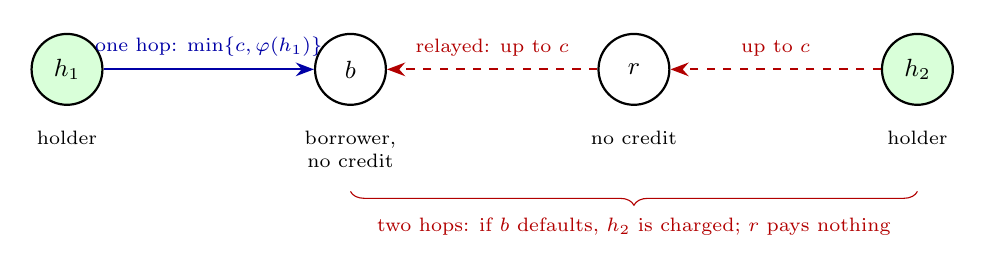
\begin{tikzpicture}[
    acct/.style={circle, draw, thick, minimum size=9mm, inner sep=0pt, font=\small},
    holder/.style={acct, fill=green!15},
    line/.style={-{Stealth[length=2.3mm]}, thick},
    lab/.style={font=\scriptsize, above=1pt},
    note/.style={font=\scriptsize, align=center, below=2mm},
  ]
  \node[holder] (h1) at (-3.6,0) {$h_1$};
  \node[acct] (b) at (0,0) {$b$};
  \node[acct] (r) at (3.6,0) {$r$};
  \node[holder] (h2) at (7.2,0) {$h_2$};
  \node[note] at (h1.south) {holder};
  \node[note] at (b.south) {borrower,\\no credit};
  \node[note] at (r.south) {no credit};
  \node[note] at (h2.south) {holder};
  \draw[line, blue!65!black] (h1) -- node[lab, text=blue!65!black] {one hop: $\min\{c,\varphi(h_1)\}$} (b);
  \draw[line, red!70!black, dashed] (r) -- node[lab, text=red!70!black] {relayed: up to $c$} (b);
  \draw[line, red!70!black, dashed] (h2) -- node[lab, text=red!70!black] {up to $c$} (r);
  \draw[decorate, decoration={brace, amplitude=5pt, mirror}, red!70!black] (0,-1.55) -- node[below=6pt, font=\scriptsize, align=center] {two hops: if $b$ defaults, $h_2$ is charged; $r$ pays nothing} (7.2,-1.55);
\end{tikzpicture}

  \caption{A borrower $b$ without credit, two of its neighbours ($r$ without credit, $h_1$ a holder) and
  a holder $h_2$ two hops away. One hop draws only $h_1$'s backing. Two hops also route $h_2$'s credit
  through $r$, which holds nothing and cannot pay if $b$ defaults; the loss falls on $h_2$, which
  never chose $b$. Under the path-liable rule $r$ can pass on nothing, and the flow is one-hop again.}
  \label{fig:regimes}
\end{figure}

Two variants of one-hop frame the protocol. \emph{One-hop-static} commits at the time of backing, as
the protocol does: each holder splits its credit evenly over its neighbours without credit before
anyone borrows. Plain one-hop commits on draw, which the protocol allows by backing and borrowing in
one transaction.

% ---------------------------------------------------------------------------------------------
\section{Two Propositions}\label{sec:props}

\begin{proposition}[Solvent intermediaries]\label{prop:pathliable}
In the path-liable regime, the maximum flow into a borrower $b$ equals the one-hop value
$\sum_{u\in N(b)}\min\{c,\varphi(u)\}$, in every state of the network.
\end{proposition}

\begin{proof}
Every unit reaching $b$ crosses an arc $(u,b)$ with $u\in N(b)$, and the flow on that arc is at most
$c$ and at most $u$'s throughput, which is at most $\varphi(u)$. So the maximum flow is at most the
one-hop value. Conversely, each neighbour $u$ can send $\min\{c,\varphi(u)\}$ from its own supply
directly to $b$, which uses $u$'s throughput only for its own credit and respects every cap. So the
one-hop value is attained.
\end{proof}

The same argument applies to a set of borrowers, with each neighbour's total into the set capped by
its free credit. The proposition holds in every state, not only on a fresh network, and it was
confirmed on 2,580 sampled borrowers (Section~\ref{sec:design}). The multi-hop networks of
\citet{karlan2009trust} escape it because intermediaries pay with social collateral, the value of
their relationships; a contract over pseudonymous accounts cannot seize that.

For attacks, let an attacker add $m$ accounts with no credit and unlimited trust among themselves,
the \emph{Sybil set} $S$, and let $g$ honest accounts each extend a line of $c$ to one of them.

\begin{proposition}[Sybil cuts]\label{prop:sybil}
In every regime of Definition~\ref{def:regimes} except the centralised one, the maximum flow into
$S$ equals the minimum cut separating the holders from $S$ in that regime's network. It does not
depend on $m$ or on the edges inside $S$, and it is at most $g\,c$. Under one-hop it is at most $c$
times the number of attack edges whose honest endpoint is a holder.
\end{proposition}

\begin{proof}
Join every account of $S$ to a super-sink with arcs of unlimited capacity. $S$ contains no supply, so
any flow into $S$ ends at the first Sybil account it reaches, and arcs inside $S$ carry nothing that
an arc into the super-sink could not. The value is therefore the maximum flow from the holders to
the super-sink in a network that does not depend on $S$'s size or internal edges, and by the
max-flow min-cut theorem \citep{ford1956} it equals the minimum cut. The $g$ attack edges form a
cut of capacity $g\,c$. Under one-hop, only a holder's own credit can cross an attack edge.
\end{proof}

The centralised lender has no bound: one Sybil account can draw all free credit. The proposition is
the credit-network form of the attack-edge bounds of SybilLimit \citep{yu2008sybillimit} and of
\citet{litos2017trust}. What differs across regimes is the constant: under multi-hop routing an
attack edge opened by an account without credit is worth up to $c$, and its cost falls on holders
behind it.

% ---------------------------------------------------------------------------------------------
\section{Experimental Design}\label{sec:design}

\paragraph{Graphs.} Watts--Strogatz small worlds \citep{watts1998} with $n$ from 500 to 2,000, mean
degree 4 to 12 and rewiring 0.05 to 0.3; Barab\'asi--Albert graphs \citep{barabasi1999} with $m$ equal
to half the degree; and a stochastic block model \citep{holland1983} with 10 equal blocks and 10\% of
each account's expected degree across blocks, run with credit anywhere and with credit only in the
first five blocks. Holder sets are nested in $q$, and the graph is shared across $q$ and $c$, so
sweeps compare like with like.

\paragraph{Base point.} $n=1{,}000$, Watts--Strogatz, mean degree 8, rewiring 0.1, $q=0.2$,
$L=100$, $c=25$ (a full line backs four neighbours), loans of $x=50$.

\paragraph{Single borrower.} On a fresh network, a random account without credit; we report the
probability that it can borrow 50 and its mean maximum, over 600 borrowers per setting (three graphs
of 200).

\paragraph{Repeated loans.} Following \citet{dandekar2011liquidity}, one request per step from a
uniformly random account without credit, for $x=50$. A granted loan draws its flow and is repaid
after a geometric number of steps, which releases the flow. The mean duration makes the open
principal, if every request succeeded, half of all issued credit, by Little's law \citep{little1961}.
After a warm-up of $\max(3D,300)$ requests we measure 2,000, with standard errors from five batches of
400; every regime faces the same request sequence. A multi-hop regime first tries direct backers, pro
rata as one-hop does, and routes a longer flow only if they fall short: for $k=2,3$ the $k$-hop flow
with the fewest arc units, and for unbounded routing Dinic's algorithm \citep{dinic1970}, which
augments along shortest paths first.

\paragraph{Computing length-bounded flows.} Two-hop flow is a plain maximum flow on a layered network
and exact. Three-hop flow is not, because an arc can sit at different positions of different paths;
we solve the time-expanded linear programme of \citet{baier2010}, whose optimum is fractional in
general (the integral problem is NP-hard). The $k$-hop programme matches explicit enumeration of every
simple path of at most $k$ arcs; unbounded flow matches an independent implementation and the
$k$-hop programme at $k=n-1$; every flow respects capacities and conserves flow; and on all 25,800
sampled borrowers the ordering one-hop-static $\le$ one-hop $\le$ 2-hop $\le$ 3-hop $\le$ unbounded
$\le$ centralised holds.

% ---------------------------------------------------------------------------------------------
\section{Results}\label{sec:results}

\subsection{How much one hop costs}

Tables~\ref{tab:fresh} and~\ref{tab:steady} report the base point. On a fresh network one hop lets a
third to a half of borrowers without credit borrow 50; every multi-hop regime serves nearly all of
them when credit is spread. Under repeated loans one hop serves 28 to 43\%, and two hops multiply that
by 1.85 to 3.05. Where credit is spread, the mean maximum a borrower can draw rises from about 40 under one
hop to over 160 under two hops, because the second hop turns the borrower's whole set of incoming lines, degree times
$c$, into capacity.

\begin{table}[ht]
  \centering\small
  \caption{Fresh network at the base point: probability that a borrower without credit can borrow
  50, by regime (``1-hop, ahead'': credit committed evenly before demand), and its mean maximum (one
  hop / two / three / unbounded).}
  \label{tab:fresh}
  \footnotesize\setlength{\tabcolsep}{3.5pt}
  \begin{tabular}{lrrrrrrl}
    \toprule
    Graph & 1-hop, ahead & 1-hop & 2-hop & 3-hop & Unbounded & Central & Mean maximum \\
    \midrule
    \inputrows{data/table_fresh.tex}
    \bottomrule
  \end{tabular}
\end{table}

\begin{table}[ht]
  \centering\small
  \caption{Steady state of repeated loans at the base point: share of requests granted (standard
  errors at most 0.006).}
  \label{tab:steady}
  \begin{tabular}{lrrrrr}
    \toprule
    Graph & One-hop & 2-hop & 3-hop & Unbounded & Centralised \\
    \midrule
    \inputrows{data/table_steady.tex}
    \bottomrule
  \end{tabular}
\end{table}

When credit is spread, the second hop is most of the gain: it closes 71 to 86\% of the steady-state
gap between one hop and unbounded routing, and the third hop closes 93 to 99\%. When credit sits in
other communities, long paths carry the gain: in the block model with credit in half the blocks, two
hops close only 36\% of the gap, three hops 68\%, and unbounded routing still adds 20 points, because
those loans cross community boundaries and every trust regime is capped by the cut between the
communities. Figure~\ref{fig:degree} shows how the cost falls as the graph gets denser.

\begin{figure}[ht]
  \centering
  % Figure: steady-state success against mean degree (data/degree_ws.csv, data/degree_sbm_half.csv).
\begin{tikzpicture}
  \begin{groupplot}[
      group style={group size=2 by 1, horizontal sep=1.4cm},
      width=0.47\linewidth, height=5cm,
      xmin=4, xmax=12, xtick={4,6,8,10,12}, ymin=0, ymax=1.05,
      xlabel={mean degree},
      tick label style={font=\footnotesize}, label style={font=\small}, title style={font=\small},
      legend style={font=\scriptsize, draw=none, fill=white, fill opacity=0.85, text opacity=1, at={(0.97,0.03)}, anchor=south east},
    ]
    \nextgroupplot[title={Watts--Strogatz}, ylabel={share of requests granted}]
    \addplot[thick, mark=*, mark size=1.2pt, blue!65!black] table[x=degree, y=s_one-hop, col sep=comma] {data/degree_ws.csv};
    \addlegendentry{one hop}
    \addplot[thick, mark=square*, mark size=1.2pt, green!45!black] table[x=degree, y=s_2-hop, col sep=comma] {data/degree_ws.csv};
    \addlegendentry{2 hops}
    \addplot[thick, mark=triangle*, mark size=1.4pt, orange!80!black] table[x=degree, y=s_3-hop, col sep=comma] {data/degree_ws.csv};
    \addlegendentry{3 hops}
    \addplot[thick, mark=diamond*, mark size=1.4pt, red!70!black] table[x=degree, y=s_unbounded, col sep=comma] {data/degree_ws.csv};
    \addlegendentry{unbounded}

    \nextgroupplot[title={SBM, credit in half the blocks}]
    \addplot[thick, mark=*, mark size=1.2pt, blue!65!black] table[x=degree, y=s_one-hop, col sep=comma] {data/degree_sbm_half.csv};
    \addplot[thick, mark=square*, mark size=1.2pt, green!45!black] table[x=degree, y=s_2-hop, col sep=comma] {data/degree_sbm_half.csv};
    \addplot[thick, mark=triangle*, mark size=1.4pt, orange!80!black] table[x=degree, y=s_3-hop, col sep=comma] {data/degree_sbm_half.csv};
    \addplot[thick, mark=diamond*, mark size=1.4pt, red!70!black] table[x=degree, y=s_unbounded, col sep=comma] {data/degree_sbm_half.csv};
  \end{groupplot}
\end{tikzpicture}

  \caption{Steady-state share of requests granted against mean degree, on Watts--Strogatz graphs
  (left) and on the block model with credit in half the blocks (right).}
  \label{fig:degree}
\end{figure}

How credit is committed matters as much as the number of hops. If holders split their credit evenly
over their neighbours ahead of demand, as committing at the time of backing invites, the probability
of borrowing 50 falls from 0.50 to 0.12 at the base point. Committing on draw recovers it without
any multi-hop routing. Figure~\ref{fig:borrowable} shows the whole distribution of what a borrower
can draw.

\begin{figure}[ht]
  \centering
  % Figure: P(maximum borrowable >= x), Watts-Strogatz base, fresh network (data/borrowable_ws.csv).
\begin{tikzpicture}
  \begin{axis}[
      width=0.72\linewidth, height=5.2cm,
      xmin=0, xmax=400, ymin=0, ymax=1.02,
      xlabel={amount $x$}, ylabel={P(can draw at least $x$)},
      tick label style={font=\footnotesize}, label style={font=\small},
      legend style={font=\scriptsize, draw=none, at={(0.97,0.97)}, anchor=north east},
    ]
    \addplot[thick, dotted, blue!65!black] table[x=x, y=one-hop-static, col sep=comma] {data/borrowable_ws.csv};
    \addlegendentry{one hop, committed ahead}
    \addplot[thick, blue!65!black] table[x=x, y=one-hop, col sep=comma] {data/borrowable_ws.csv};
    \addlegendentry{one hop}
    \addplot[thick, green!45!black] table[x=x, y=2-hop, col sep=comma] {data/borrowable_ws.csv};
    \addlegendentry{2 hops}
    \addplot[thick, orange!80!black] table[x=x, y=3-hop, col sep=comma] {data/borrowable_ws.csv};
    \addlegendentry{3 hops}
    \addplot[thick, red!70!black] table[x=x, y=unbounded, col sep=comma] {data/borrowable_ws.csv};
    \addlegendentry{unbounded}
  \end{axis}
\end{tikzpicture}

  \caption{Probability that a borrower without credit can draw at least $x$, Watts--Strogatz base
  point, fresh network.}
  \label{fig:borrowable}
\end{figure}

\subsection{The same service from more credit}

In a protocol whose lenders' worst-case loss is the issued credit \citep{conservedcredit2026}, the
natural price of the one-hop rule is the extra credit it needs for the same service. On the
Watts--Strogatz base graph we run one hop on a fine grid of $q$ and find the issued credit it needs to
reach each regime's success at $q=0.2$ (Table~\ref{tab:equivalence}, Figure~\ref{fig:equivalence}).
In the steady state one hop needs 2.1 times the issued credit to match two hops, 3.1 times to match
three and 3.8 times to match unbounded routing.

\begin{table}[ht]
  \centering\small
  \caption{Issued credit one hop needs to match each regime at $q=0.2$ (Watts--Strogatz base graph;
  targets capped at 99\%).}
  \label{tab:equivalence}
  \begin{tabular}{lrrrrrr}
    \toprule
    & \multicolumn{3}{c}{Fresh network} & \multicolumn{3}{c}{Steady state} \\
    \cmidrule(lr){2-4}\cmidrule(lr){5-7}
    Regime at $q=0.2$ & Success & One hop needs $q$ & Multiple & Success & One hop needs $q$ & Multiple \\
    \midrule
    \inputrows{data/table_equivalence.tex}
    \bottomrule
  \end{tabular}
\end{table}

\begin{figure}[ht]
  \centering
  % Figure: one-hop success against q, with multi-hop steady-state success at q = 0.2
% (data/equivalence_curve.csv; horizontal lines from Table 3).
\begin{tikzpicture}
  \begin{axis}[
      width=0.72\linewidth, height=5.2cm,
      xmin=0.05, xmax=0.8, ymin=0, ymax=1.05,
      xlabel={share of accounts holding a line, $q$}, ylabel={one-hop success},
      tick label style={font=\footnotesize}, label style={font=\small},
      legend style={font=\scriptsize, draw=none, at={(0.97,0.03)}, anchor=south east},
    ]
    \addplot[thick, blue!65!black, mark=*, mark size=1pt] table[x=q, y=onehop_static, col sep=comma] {data/equivalence_curve.csv};
    \addlegendentry{one hop, fresh}
    \addplot[thick, dashed, blue!65!black, mark=o, mark size=1pt] table[x=q, y=onehop_steady, col sep=comma] {data/equivalence_curve.csv};
    \addlegendentry{one hop, steady}
    \addplot[thin, green!45!black, domain=0.05:0.8] {0.828};
    \addlegendentry{2 hops at $q=0.2$, steady}
    \addplot[thin, orange!80!black, domain=0.05:0.8] {0.958};
    \addlegendentry{3 hops at $q=0.2$, steady}
    \addplot[dotted, gray] coordinates {(0.2,0) (0.2,1.05)};
  \end{axis}
\end{tikzpicture}

  \caption{One-hop success as the share of holders $q$ grows (fresh and steady state), against the
  steady-state success of the multi-hop regimes at $q=0.2$ (horizontal lines).}
  \label{fig:equivalence}
\end{figure}

\subsection{Who stands behind a multi-hop loan}

Proposition~\ref{prop:pathliable} says the multi-hop gain must come from relays that cannot pay.
Table~\ref{tab:liability} measures it in the steady state. Half to five-sixths of granted two-hop
loans need a path longer than one arc; 40 to 62\% of two-hop volume enters the borrower from an
account with no credit; and 37 to 66\% is supplied by holders not adjacent to the borrower, who are
charged if it defaults although they never chose it. Under unbounded routing these shares rise to 53
to 72\% and 50 to 75\%. The storage a routed loan touches on chain, one slot per source and per arc,
is modest for two and three hops and grows only for unbounded routing on community graphs.

\begin{table}[ht]
  \centering\small
  \caption{Steady state at the base point. Routed: granted loans that needed a path longer than one
  arc. Relayed: share of volume entering the borrower from an account without credit. Remote: share
  supplied by holders not adjacent to the borrower. Slots: storage slots a routed loan touches.}
  \label{tab:liability}
  \begin{tabular}{llrrrrr}
    \toprule
    Graph & Regime & Routed & Mean hops & Relayed & Remote & Slots \\
    \midrule
    \inputrows{data/table_liability.tex}
    \bottomrule
  \end{tabular}
\end{table}

\subsection{Sybil extraction}

Table~\ref{tab:sybil} reports what $m=1$ Sybil account extracts behind $g$ attack edges on the
Watts--Strogatz base graph; every value is identical for $m=1$, 10, 100 and 1,000, and equals the
regime's cut, as Proposition~\ref{prop:sybil} states. With attack edges from random accounts, one hop
yields only the edges whose endpoint is a holder, while two or more hops yield nearly $g\,c$. Edges
from accounts without credit are worth nothing under one hop and the full $g\,c$ under routing. With
random endpoints, $q=0.2$ and $g\ge20$, the same attack edges extract 3.3 to 7 times as much under
multi-hop routing as under one hop, across the three graph families, and 66 to 100\% of it is charged
to holders that never trusted a Sybil account.

\begin{table}[ht]
  \centering\small
  \caption{Extraction by Sybil accounts behind $g$ attack edges of capacity $c=25$ (Watts--Strogatz
  base graph); ``Holders'' counts attack edges whose honest endpoint holds credit. The values are
  identical for 1, 10, 100 and 1,000 Sybil accounts.}
  \label{tab:sybil}
  \footnotesize\setlength{\tabcolsep}{3.5pt}
  \begin{tabular}{lrrrrrrrr}
    \toprule
    Attack edges from & $g$ & Holders & $g\,c$ & 1-hop & 2-hop & 3-hop & Unbounded & Path-liable \\
    \midrule
    \inputrows{data/table_sybil.tex}
    \bottomrule
  \end{tabular}
\end{table}

% ---------------------------------------------------------------------------------------------
\section{Discussion}\label{sec:discussion}

\paragraph{The trade-off.} Multi-hop routing roughly doubles liquidity for borrowers without credit
at realistic densities, at little cost in on-chain storage. It is not free in the currency a lending
protocol cares about: it exists only because intermediaries can pass on credit they could not pay
for, and it charges defaults to accounts that did not choose the borrower. A protocol that rests on
backers bearing the loss of their own choice gives up exactly that link.

\paragraph{Two design options.} If routing is added, two choices keep most of its gain and make its
liability explicit: limit paths to two hops, which captures 71 to 86\% of the gain when credit is
spread, and make relaying a permission that each holder grants per line, so a holder that does not
opt in keeps one-hop liability and one that does underwrites its neighbours' choices knowingly.
Before either, committing backing on draw rather than ahead of demand recovers the liquidity lost to
pre-commitment at no change in liability.

\paragraph{Limits.} Trust is uniform and symmetric, and every holder extends lines to all its
neighbours; real backers choose, so the one-hop figures are an upper bound for a protocol in which
backing is committed in advance. Holders have equal lines and do not borrow. Borrowers ask for a fixed
amount and take all or nothing. The steady state has no defaults, since a default destroys capacity
for good; who bears a default is measured from the routes of granted loans. The routing policy is one
reasonable choice among several. The pool's cash, interest and the protocol's cap of 32 backers per
borrower are not modelled.

\paragraph{Open questions.} Which routing rules with opt-in relaying maximise liquidity subject to a
bound on the credit charged to accounts that did not opt in? And how do holders choose whom to back
when their credit is at stake, which this paper takes as given?

\section{Conclusion}

Restricting a credit network to one hop costs about half of the liquidity available to borrowers
without credit, or two to four times the issued credit for the same service. The restriction is
exactly the requirement that every intermediary be able to pay for what it passes on, so the cost is
the price of keeping liability with the accounts that chose the borrower. Two-hop routing with opt-in
relaying is the natural middle ground.

\paragraph{Disclosure of AI authorship.} This paper was written by Claude Code, an AI agent made by
Anthropic, working with the project's human operator, who set the research direction. The simulation
code was written by AI agents working with the project. All of it is public and reproducible.

{\sloppy\paragraph{Data and code availability.} The experiments are in \texttt{analysis/liquidity} of
\url{https://github.com/scottonchain/microcredit-contract} at commit b725a85; the script that extracts
every table and figure is in \url{https://github.com/scottonchain/microcredit-theory}.\par}

\bibliographystyle{apalike}
\bibliography{references}

\end{document}
